\chapter{Конструкторский раздел}

\section{Функциональные требования к протоколу}

Ниже перечислены функциональные требования к разрабатываемому протоколу.

\begin{enumerate}
    \item Протокол должен поддерживать проведение одной конференции для произвольного количества участников.
    \item Участники должны иметь возможность подключаться и отключаться от конференции во время ее проведения.
\end{enumerate}

\section{Роли участников конференции}

При создании конференции участник, который ее создает (и отправляет приглашения остальным участникам) назначается управляющим конференцией.

Управляющий конференцией имеет возможность редактировать параметры конференции, рассылать приглашения, а также передать свои полномочия другому участнику конференции.

Протокол не предусматривает четкого списка ролей.

\section{Типы сообщений}

Разрабатываемый протокол предусматривает следующие типы сообщений:
\begin{itemize}[label=---]
    \item \texttt{INVITE} (0) --- приглашение в конференцию. Получатель сообщения подключается к конференции, в которой участвует отправитель.
    \item \texttt{INVITE\_ACCEPT} (1) --- участник принимает приглашение.
    \item \texttt{INVITE\_REJECT} (2) --- участник отклоняет приглашение.
    \item \texttt{PART\_PRESENCE} (3) --- подключение/отключение участников конференции.
    \item \texttt{PART\_INFO} (4) --- изменение состояния отдельного участника конференции.
    \item \texttt{REENTER} (5) --- отправитель намеревается подключиться к существующей конференции (после потери соединения).
    \item \texttt{LEAVE} (6) --- отправитель намеривается покинуть конференцию. Получатели должны финализировать все ресурсы, связанные с этим участником и разорвать соединения. Без использования данного типа сообщения будет происходить ожидание переподключения участника.
    \item \texttt{TEXT} (7) --- текстовое сообщение.
    \item \texttt{AUDIO} (8) --- сообщение с аудио пакетом.
    \item \texttt{VIDEO} (9) --- сообщение с видео пакетом.
\end{itemize}

Для передачи данных между участниками используется бинарный формат сообщений.

Схема типов сообщений представлена в таблицах \ref{tbl:msg:invite}---\ref{tbl:msg:video}.
Первым полем любого сообщения передается его размер, затем поле с типом сообщения, в зависимости от которого происходит анализ содержимого сообщения.

Идентификаторы конференций и участников генерируются случайным образом.

\begin{table}[H]
  \centering
  \caption{Структура сообщения типа \texttt{INVITE}}
  \label{tbl:msg:invite}
  \begin{tabular}{|l|l|l|}
    \hline
    \textbf{Поле} & \textbf{Размер} & \textbf{Описание} \\ \hline
    \texttt{size} & 8 байт & Размер сообщения, равен 36 + N \\ \hline
    \texttt{type} & 4 байт & Тип сообщения, равен 0 \\ \hline
    \texttt{conf\_id} & 8 байт & Идентификатор конференции \\ \hline
    \texttt{part\_id} & 8 байт & Идентификатор приглашающего участника \\ \hline
    \texttt{conf\_start\_ts} & 8 байт & Временная метка UTC начала конференции \\ \hline
    \texttt{part\_name} & N байт & Строковое имя приглашающего участника \\ \hline
  \end{tabular}
\end{table}

\begin{table}[H]
  \centering
  \caption{Структура сообщения типа \texttt{INVITE\_ACCEPT}}
  \label{tbl:msg:invite-accept}
  \begin{tabular}{|l|l|l|}
    \hline
    \textbf{Поле} & \textbf{Размер} & \textbf{Описание} \\ \hline
    \texttt{size} & 8 байт & Размер сообщения, равен 20 + N \\ \hline
    \texttt{type} & 4 байт & Тип сообщения, равен 1 \\ \hline
    \texttt{part\_id} & 8 байт & Идентификатор присоединившегося участника \\ \hline
    \texttt{part\_name} & N байт & Строковое имя приглашенного участника \\ \hline
  \end{tabular}
\end{table}

\begin{table}[H]
  \centering
  \caption{Структура сообщения типа \texttt{INVITE\_REJECT}}
  \label{tbl:msg:invite-reject}
  \begin{tabular}{|l|l|l|}
    \hline
    \textbf{Поле} & \textbf{Размер} & \textbf{Описание} \\ \hline
    \texttt{size} & 8 байт & Размер сообщения, равен 12 \\ \hline
    \texttt{type} & 4 байт & Тип сообщения, равен 2 \\ \hline
  \end{tabular}
\end{table}

\begin{table}[H]
  \centering
  \caption{Структура сообщения типа \texttt{PART\_PRESENCE}}
  \label{tbl:msg:part-presence}
  \begin{tabular}{|l|l|l|}
    \hline
    \textbf{Поле} & \textbf{Размер} & \textbf{Описание} \\ \hline
    \texttt{size} & 8 байт & Размер сообщения, равен 28 \\ \hline
    \texttt{type} & 4 байт & Тип сообщения, равен 3 \\ \hline
    \texttt{part\_id} & 8 байт & Идентификатор участника \\ \hline
    \texttt{part\_role} & 4 байт & Роль участника \\ \hline
    \texttt{state} & 4 байт & 0 --- участник присоединился; \\
    & & 1 --- иначе \\ \hline
  \end{tabular}
\end{table}

\begin{table}[H]
  \centering
  \caption{Структура сообщения типа \texttt{PART\_INFO}}
  \label{tbl:msg:part-info}
  \begin{tabular}{|l|l|l|}
    \hline
    \textbf{Поле} & \textbf{Размер} & \textbf{Описание} \\ \hline
    \texttt{size} & 8 байт & Размер сообщения, равен 24 + N \\ \hline
    \texttt{type} & 4 байт & Тип сообщения, равен 4 \\ \hline
    \texttt{part\_id} & 8 байт & Идентификатор участника \\ \hline
    \texttt{part\_role} & 4 байт & Новая роль участника \\ \hline
    \texttt{part\_name} & N байт & Новое строковое имя участника \\ \hline
  \end{tabular}
\end{table}

\begin{table}[H]
  \centering
  \caption{Структура сообщения типа \texttt{REENTER}}
  \label{tbl:msg:reenter}
  \begin{tabular}{|l|l|l|}
    \hline
    \textbf{Поле} & \textbf{Размер} & \textbf{Описание} \\ \hline
    \texttt{size} & 8 байт & Размер сообщения, равен 28 \\ \hline
    \texttt{type} & 4 байт & Тип сообщения, равен 5 \\ \hline
    \texttt{conf\_id} & 8 байт & Идентификатор конференции \\ \hline
    \texttt{part\_id} & 8 байт & Идентификатор перезаходящего участника \\ \hline
  \end{tabular}
\end{table}

\begin{table}[H]
  \centering
  \caption{Структура сообщения типа \texttt{LEAVE}}
  \label{tbl:msg:leave}
  \begin{tabular}{|l|l|l|}
    \hline
    \textbf{Поле} & \textbf{Размер} & \textbf{Описание} \\ \hline
    \texttt{size} & 8 байт & Размер сообщения, равен 20 \\ \hline
    \texttt{type} & 4 байт & Тип сообщения, равен 6 \\ \hline
    \texttt{part\_id} & 8 байт & Идентификатор уходящего участника \\ \hline
  \end{tabular}
\end{table}

\begin{table}[H]
  \centering
  \caption{Структура сообщения типа \texttt{TEXT}}
  \label{tbl:msg:text}
  \begin{tabular}{|l|l|l|}
    \hline
    \textbf{Поле} & \textbf{Размер} & \textbf{Описание} \\ \hline
    \texttt{size} & 8 байт & Размер сообщения, равен 20 + N \\ \hline
    \texttt{type} & 4 байт & Тип сообщения, равен 7 \\ \hline
    \texttt{part\_id} & 8 байт & Идентификатор участника--источника \\ \hline
    \texttt{text} & N байт & Текстовое сообщение \\ \hline
  \end{tabular}
\end{table}

\begin{table}[H]
  \centering
  \caption{Структура сообщения типа \texttt{AUDIO}}
  \label{tbl:msg:audio}
  \begin{tabular}{|l|l|l|}
    \hline
    \textbf{Поле} & \textbf{Размер} & \textbf{Описание} \\ \hline
    \texttt{size} & 8 байт & Размер сообщения, равен 20 + N \\ \hline
    \texttt{type} & 4 байт & Тип сообщения, равен 8 \\ \hline
    \texttt{part\_id} & 8 байт & Идентификатор участника--источника \\ \hline
    \texttt{packet} & N байт & Аудио пакет \\ \hline
  \end{tabular}
\end{table}

\begin{table}[H]
  \centering
  \caption{Структура сообщения типа \texttt{VIDEO}}
  \label{tbl:msg:video}
  \begin{tabular}{|l|l|l|}
    \hline
    \textbf{Поле} & \textbf{Размер} & \textbf{Описание} \\ \hline
    \texttt{size} & 8 байт & Размер сообщения, равен 20 + N \\ \hline
    \texttt{type} & 4 байт & Тип сообщения, равен 9 \\ \hline
    \texttt{part\_id} & 8 байт & Идентификатор участника--источника \\ \hline
    \texttt{packet} & N байт & Видео пакет \\ \hline
  \end{tabular}
\end{table}

\section{Медиа форматы}

Снижение объемов передачи аудио/видео данных по сети требует использования кодеков, сжимающих медиа данные. Для разрабатываемого протокола применяются кодеки AAC \cite{aac} и H.264 \cite{h264}. Аудио кадр кодируется в стерео формате с частотой 48кГц. Видео кадр кодируется в разрешении 320 на 180 пикселей и частотой в 30 кадров в секунду.

Закодированный аудио/видео кадр записывается в поле \texttt{packet} сообщений \texttt{AUDIO}/\texttt{VIDEO}.

\section{Взаимодействия сторон}

Рассмотрим сценарий с двумя участниками --- <<А>> и <<Б>>.
При создании конференции ей назначается случайный идентификатор. Для организации конференции, участник <<А>> отправляет участнику <<Б>> сообщение типа \texttt{INVITE}, в котором записывается идентификатор конференции, а также идентификатор и имя приглашающего участника.
После чего участник <<Б>> должен ответить на него сообщением \texttt{INVITE\_ACCEPT} для подключения к конференции участника <<А>>, при этом он покидает свою текущую конференцию, если ее идентификатор не совпадает с идентификатором конференции в приглашении.
После успешного подключения, происходит инициализация каналов передачи медиа данных.

\begin{figure}[H]
  \centering
  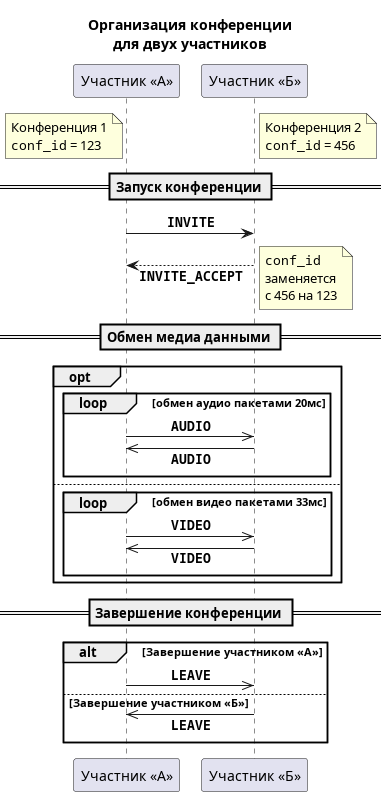
\includegraphics[width=0.5\linewidth]{inc/diag/seq-2/conf-2.png}
  \caption{Диаграмма последовательности для организации конференции для двух участников}
  \label{img:conf-2}
\end{figure}

Аудио и видео пакеты передаются с использованием сообщений типов \texttt{AUDIO} / \texttt{VIDEO}.
Диаграмма последовательности описанного процесса представлена на рисунке \ref{img:conf-2}.

Подключение последующих участников происходит аналогичным образом --- любой из активных участников конференции отправляет сообщение типа \texttt{INVITE} с приглашением в конференцию новому участнику, и, после получения ответного сообщения \texttt{INVITE\_ACCEPT}, отправляет сообщение \texttt{PART\_PRESENCE} остальным участникам конференции для уведомления о подключении нового участника.
Каждый из остальных участников, получив сообщение \texttt{PART\_PRESENCE} отправляет приглашение \texttt{INVITE} новому участнику для инициализации каналов связи между всеми парами участников конференции.
Диаграмма последовательности описанного процесса представлена на рисунке \ref{img:conf-3}.

\begin{figure}[H]
  \centering
  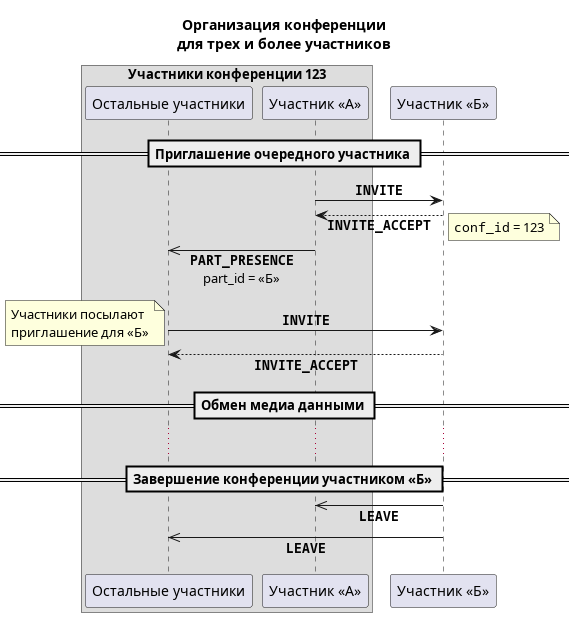
\includegraphics[width=0.9\linewidth]{inc/diag/seq-3/conf-3.png}
  \caption{Диаграмма последовательности для организации конференции для трех и более участников}
  \label{img:conf-3}
\end{figure}

Для обеспечения уникальной идентификации участников в условиях, когда несколько клиентов могут находиться за NAT с одним IP-адресом, в протоколе используются уникальные идентификаторы участников.
Эти идентификаторы генерируются случайным образом при подключении участника к конференции и используются для однозначной идентификации в рамках сессии.

\section{Шифрование}

Шифрование используется для обеспечения целостности и конфиденциальности передаваемых данных. (Защита от подслушивания, порчи и/или подделки сообщений).
Проверка сертификатов разрабатываемым протоколом не предусмотрена, но может быть проведена при повторном соединении с участником.
В качестве протокола шифрования используется TLS v1.3 \cite{tls}.

%В итоге, выбор между TCP+TLS и SRTP зависит от конкретных требований проекта. TCP+TLS лучше подходит для приложений, где важны надежность, безопасность и совместимость, в то время как SRTP более эффективен для передачи мультимедийных данных с низкой задержкой. Важно также учитывать ресурсные ограничения целевых платформ и сложность реализации каждого из подходов.

\section{Переподключение}

При потере соединения без получения сообщения \texttt{LEAVE} небходимо ожидать переподключение участника в течении 30 секунд. Если участник так и не подключился к конференции, то он считается вышедшим из конференции и в последующем сможет подключиться к ней только через приглашение от другого участника конференции.

Переподключение производится отправкой сообщения \texttt{REENTER} с идентификатором текущей конференции и идентификатором участника, потерявшего соединение. Если сообщение было получено по истечению 30 секундного интервала --- оно отбрасывается, соединение закрывается и участник считывается неподключившимся.

\section{Определение качества каналов связи}

Для реформирования топологии связей в бессерверных видео конференциях необходимо определить качество существующих каналов связи между участниками. Это может быть выполнено с использованием метрик, которые зависят от следующих параметров: временные метки отправки/приема аудио/видео пакета; размер пакета в байтах; количество переданных и повторно переданных пакетов.

На основе этих параметров могут быть вычислены такие показатели качества как:
\begin{itemize}[label=---]
  \item задержка передачи --- временная разница между отправкой и получением пакета;
  \item джиттер --- вариация задержки между последовательными пакетами;
  \item пропускная способность --- объем данных, переданных за определенный период времени.
\end{itemize}
